\documentclass{my_Presentation}

\title{Agiles Softwaremanagement}
\author{Koch, Merkl, Pfitzner}
%\institute{Mobile Robotic Laboratory}
\date{\today}



\begin{document}
%##################################################
\frame{\titlepage \vspace{-0.5cm}
\begin{center}
	\includegraphics[scale=0.5]{Ohm.pdf}\\
	Technische Hochschule Nurnberg
\end{center}
}
%%~~~~~~~~~~~~~~~~~~~~~~~~~~~~~~~~~~~~~~~~~~~~~~~~~~~
\frame{
	\frametitle{Content}
	\begin{minipage}[b]{0.47\linewidth}
		\tableofcontents[pausesection]
	\end{minipage}
}

%%##################################################
\section{Organisation}
\frame{
\frametitle{Teilnehmer}
	\begin{itemize}
		\item \textbf{Stefan May:} Product Owner
		\item \textbf{Philipp Koch:} Scrum Master
		\item \textbf{Christian Merkl:} Teammitglied
		\item \textbf{Christian Pfitzner:} Teammitglied
	\end{itemize}		
	\vfill
	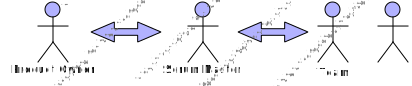
\includegraphics[width=0.9\textwidth]{../grafiken/Team.pdf}
 
}
%%##################################################
%introuserstories
%Einleitende user story -> phil

\frame{
\frametitle{App}
  \begin{block}{User Stories}
   \begin{itemize}
   \item Das zu entwerfende Produkt ist eine App, die von ausländischen Studenten verwendet kann, um sich an der TH und in der umgebenden Stadt zurecht zu finden.
   \item Die App soll auf jedem beliebigen Android Gerät laufen.
   \item Die App soll in Java programmiert werden.
   \item Das Design der Menus und aller Widgets soll dem Design und den Farben der Homepage der TH folgen.
   \item Bei der Programmierung sollen soweit möglich vorhandene Bibliotheken und Werkzeuge verwendet werden zurückgegriffen werden.
   \end{itemize}
  \end{block}
}

%%##################################################
\frame{
\frametitle{Zeitplan}
	Gantt Diagramm
}

\section{Das Produkt}
\frame{
\frametitle{Das Produkt}
	\begin{block}{Eine grobe Idee}
		\begin{itemize}
			\item Handy-App
			\item Plattform für internationale Studenten
			\item Wichtige Informationen auf einen Blick
			\item Kommunikation untereinander
		\end{itemize}
	\end{block}
	\begin{flushright}
			\includegraphics[width=0.5\textwidth]{../grafiken/s_handy.jpg}
	\end{flushright}
}

%%##################################################
\section{Sprint 1}
%Sprint 1 user Story & Ablauf -> Phil
\frame{
\frametitle{User Stories}
  \begin{block}{User Stories}
   \begin{itemize}
   \item \textbf{Design: } \textit{Ich wünsche mir ein Menü, dass in Farbe und Form der Homepage meiner Hochschule ähnelt.}
   \item \textbf{Bedienelemente:} \textit{Die Bedienungsknöpfe sollen links untereinander angebracht sind, am Boden soll eine Statusleiste die aktuelle Informationen enthalten.}
   \item \textbf{Benutzerfoto: } \textit{Im Hauptmenü soll ein Foto des Benutzers angezeigt werden.}
   \item \textbf{Funktionalität:} \textit{Ich möchte die Grundfunktionalität anhand von Dummyfunktionen sehen. }
   \end{itemize}
 \end{block}
}
\frame{
\frametitle{Planung}
  \begin{block}{Sprint Backlog}
   \begin{itemize}
   \item Design des Hauptmenu
    \item Design des Startbildes
    \item Implementierung der Grundfunktionalität (Dummy-Funktionen)
   \end{itemize}
  \end{block}  
}
%%~~~~~~~~~~~~~~~~~~~~~~~~~~~~~~~~~~~~~~~~~~~~~~~~~~~
\frame{
\frametitle{GUI: Programmaufbau}
	\begin{block}{Anforderungen}
		\begin{itemize}
			\item Basisklasse GUI enthält mögliche Designelemente für einzelne Abschnitte der APP
			\item Seiten erben von Basisklasse und implementieren eigene Funktionalität
		\end{itemize}
	\end{block}
}

\frame{
\frametitle{Gui: Klassendiagramm}
	\begin{center}
		\begin{figure}
			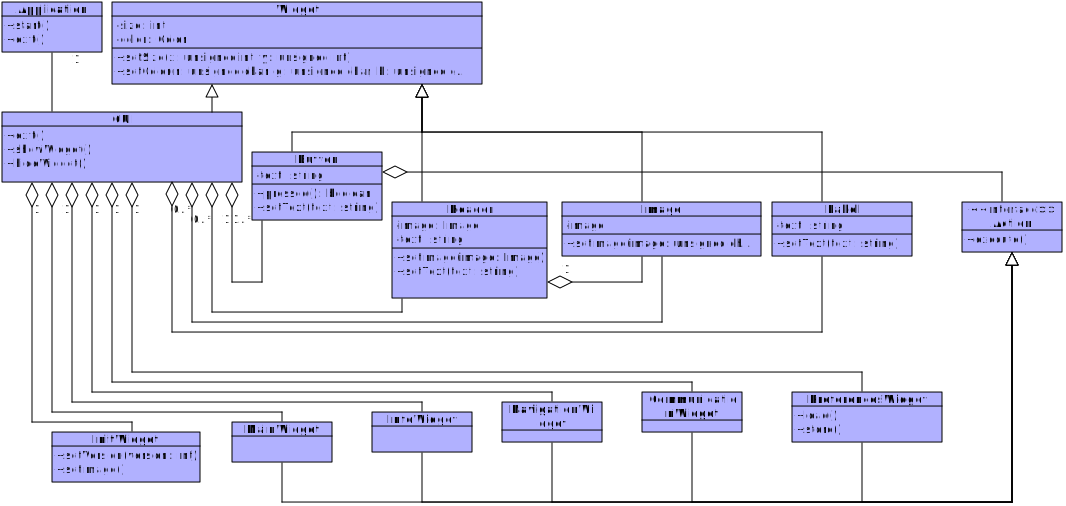
\includegraphics[width=1.0\textwidth]{../grafiken/GUI_Class.pdf}
			\caption{Klassendiagramm für Programmstruktur. }		
		\end{figure}
	\end{center}
}

\frame{
\frametitle{Menüwechsel}
	\begin{block}{Zustandsmaschine}
		\begin{itemize}
			\item \textbf{Menüpunkte} werden als \textbf{Zustand} gesehen
			\item zusätzliche Zustände für \textbf{Start und Beenden} der Application
			\item Zustände können wiederum Unter-Zustände besitzen
		\end{itemize}
		\begin{center}
			\begin{figure}
				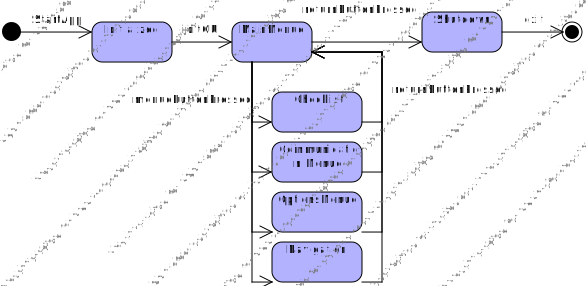
\includegraphics[width=0.55\textwidth]{../grafiken/MenueStates.pdf}
				\caption{State Machine ausgelöst durch das Interface \textit{Action}}
			\end{figure}
		\end{center}
	\end{block}
}

\begin{frame}
	\frametitle{Sprint 1 Design GUI}

	\begin{figure}
		\centering
		\includegraphics[width = 0.75\textwidth]{gui-design}
		\caption{Konzeptzeichnung für das GUI}
	\end{figure}
\end{frame}


%%##################################################

\section{Sprint 2}
%Sprint 1 user Story & Ablauf -> Phil
\frame{
\frametitle{Kartenwidget}
  \begin{block}{User Stories}
   \begin{itemize}
   \item \textbf{Lageplan TH: } \textit{Die App soll den Lageplan der Hochschule mit allen wichtigen Orten anzeigen.}
   \item \textbf{Google Maps: } \textit{Die App soll eine Schnittstelle zu Google Maps enthalten. }
   \item \textbf{Interaktive Liste: } \textit{Der Nutzer soll Zugriff auf eine von ihm veränderbare Liste mit für ihn interessanten Orten haben. }
    \end{itemize}
 \end{block}
}

\frame{
\frametitle{Kartenwidget}
  \begin{block}{Sprint Backlog}
   \begin{itemize}
  	\item Lageplan der TH integrieren
    \item Interface zu Google-maps implementieren
    \item Implementierung interaktiver Liste für Kartenwidget
    \item Übergabe von Orten aus der Liste zu Google Maps
    \end{itemize}
  \end{block}
}

\frame{
\frametitle{Navigation: Struktur}
	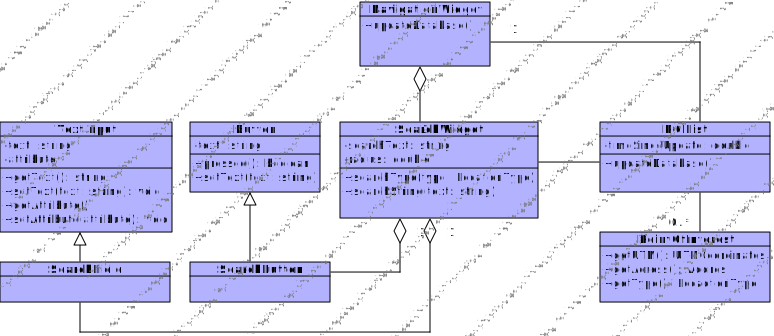
\includegraphics[width=0.9\textwidth]{../grafiken/NavigationW_Class.pdf}
}

\frame{
\frametitle{Interessantes}
	\begin{block}{Struktur}
	\begin{itemize}
		\item Basisklasse für interessante Objekte 
		\item Addressinformation für schnelles finden von Orten in der Umgebung
		\item UTM-Koordinaten zur Übergabe an Routenplanner
	\end{itemize}
	\begin{center}
		\includegraphics[width=0.8\textwidth]{../grafiken/PointOfInteresst.pdf}
	\end{center}
	\end{block}
}

%\begin{frame}
%	\frametitle{Google Map API}
%%
%	\begin{block}{Implementierung in GUI}
%		\begin{itemize}
%			\item Es existiert nur eine API für \textit{Andriod}
%			\item Workaround über Browser möglich
%			\item Ansatz: Firefox in GUI integrieren
%			\item Problem: Bläht das Programm \textbf{enorm} auf
%		\end{itemize}
%	\end{block}
%%
%	\begin{block}{Kommunikation zu SM}
%		\begin{itemize}
%			\item Problem dem Scrum Master erläutert
%			\item Klärung mit Product Owner erforderlich
%		\end{itemize}
%	\end{block}
%\end{frame}
%
%
%
\begin{frame}
	\frametitle{Lageplan der Hochschule}
%
\begin{minipage}[t]{0.48\textwidth}
	\begin{block}{Implementierung in GUI}
		\begin{itemize}
			\item \textbf{Lageplan} kann als Bild hinterlegt werden
			\item Einfache Wartung möglich
			\item Anzeige über die Klasse Image
		\end{itemize}
	\end{block}
\end{minipage}
\begin{minipage}[t]{0.48\textwidth}
	\begin{figure}
		\includegraphics[width=\textwidth]{../grafiken/lageplan.png}
		\caption{Lageplan der Hochschule Nürnberg.}
	\end{figure}
\end{minipage}
\end{frame}
%
%
%
\begin{frame}
	\frametitle{Interaktive Liste}
%
	\begin{minipage}{0.49\textwidth}
		\begin{figure}
			\centering
			\includegraphics[width = \textwidth]{../grafiken/uml-list-widget}
			\caption{UML Diagram ListWidget}
		\end{figure}
	\end{minipage}
%
	\begin{minipage}{0.44\textwidth}
		\begin{block}{ListItem}
			\begin{itemize}
			    \item Erbt von Widget
			    \item ListAction ist das Interface zum Model
			    \item ListItem enthält alle Daten für ein Item
			    \item Leicht erweiterbar
			\end{itemize}
		\end{block}
	\end{minipage}
\end{frame}

%%##################################################

\section{Sprint 3}
%Sprint 3 user Story & Ablauf -> Phil
\frame{
\frametitle{Sprint 3 Kommunikation - User Stories}
  \begin{block}{User Stories}
   \begin{itemize}
   \item Story 1 - TH-Email / Kalender
   
   Die App soll eine Möglichkeit bieten, auf die Email- und Kalenderfunktionen der TH zuzugreifen.
  
   \item Story 2 - Popup
   
   Ein Popup soll Termine anzeigen, die in einem, im Optionsmenu einstellbaren, Zeitraum liegen. 
   \item Story 3 - Checklistenwidget
   
   Die App soll eine interaktive Checkliste enthalten, in die der Nutzer Aufgaben u. Ä. eintragen kann.
   \end{itemize}
 \end{block}
}

\frame{
\frametitle{Sprint 3 Kommunikation - Planung}
  \begin{block}{Extraktion aus Product Backlog}
    \begin{itemize}
    \item Schnittstelle zu TH-Email / Kalender implementieren
    \item Popup fuer akute Termine implementieren 
    \item Implementierung des Checklistenwidgets
    \item Design des Checklistenwidgets erstellen
    \end{itemize}
  \end{block}  

}
%##################################################
\frame{
\frametitle{Email- und Kalenderanbindung}
	\begin{block}{Kommunikation mit Hochschul-Content}
		\begin{itemize}
			\item Hochschul-interne Daten über Content System für \textbf{Kalender} und \textbf{Email}
			\item Content-Zugriff und \textbf{Update bei Internetzugriff} des Mobilfunktgeräts
		\end{itemize}
	 \begin{minipage}{0.6\linewidth}
  		\includegraphics[width=0.9\textwidth]{../grafiken/OhmCollab.pdf}
    \end{minipage}
    \begin{minipage}{0.38\linewidth}
        \includegraphics[width=1.0\textwidth]{../grafiken/myOhm.png}
    \end{minipage}
    	\end{block}
}

\frame{
\frametitle{Setup Skript}
	\begin{block}{Einrichten des Ohm Content}
	\begin{itemize}
		\item Standardapplikationen von Android für Email und Kalender werden genutzt
		\item \textbf{Installationsskript} soll das Einrichten aller Ohm Content Applicationen erleichtern
		\item Daten, die der Benutzer eingeben muss: 
		\begin{itemize}
			\item Benutzername
			\item Passwort
		\end{itemize}
		\item \textbf{Serveradresse und Port} sind hochschulabhängig und hinterlegt
	\end{itemize}
	\end{block}
}

\frame{
\frametitle{Änderung des Logos}
	\begin{block}{Redesign}
		\begin{itemize}
			\item Logos im Programm im PNG-Format hinterlegt
			\item Pfade oder Namen zu Bilder müssen angepasst werden
			\item \textbf{geringer Änderungsaufwand}
		\end{itemize}
	\end{block}
}
%
%\frame{
%\frametitle{Datenhaltung}
%	\begin{block} {Content Management System (CMS)}
%	\begin{itemize}
%		\item CMS zum Verwalten von Inhalten
%		\item Verschiedene Benutzerrollen:	
%			\begin{itemize}
%				\item Administrator: Bearbeitung von Design und Inhalt
%				\item Redakteuer: Bearbeitung von Inhalt
%			\end{itemize}
%		\item $\rightarrow$ Hochschule benutzt bereits CMS-Systeme für Inhalte der Webseite. \\\textbf{Vorteil: zusätzliche Schulung nicht notwendig} 
%	\end{itemize}
%	\end{block}
%	\begin{block}{Diagramm}
%		\includegraphics[width=1.0\textwidth]{../grafiken/DB.pdf}
%	\end{block}
%}



\begin{frame}
	\frametitle{Design Popup Fenster}
%
	\begin{figure}
		\centering
		\includegraphics[width = 0.6\textwidth]{../grafiken/popup-fenster}
		\caption{Design Popup Fenster}
	\end{figure}
\end{frame}
%
%
%
\begin{frame}
	\frametitle{Design ListWidget}
%
	\begin{minipage}{0.49\textwidth}
		\begin{figure}
			\centering
			\includegraphics[height = 0.7\textheight]{../grafiken/list-widget-design}
			\caption{Design Checklisten Widget}
		\end{figure}	
	\end{minipage}
%
	\begin{minipage}{0.44\textwidth}
		\begin{block}{ListWidget}
			\begin{itemize}
				\item Enthält zwei Buttons mit Icons
				\item Zwischen den Buttons steht Text
				\item Mit Button rechts, Eintrag löschen
				\item Mit Button links, Eintrag abhacken
			\end{itemize}
		\end{block}
	\end{minipage}
\end{frame}
%
%
%
\begin{frame}
	\frametitle{Anpassung Klassenstruktur ListWidget}
%
	\begin{figure}
		\centering
		\includegraphics[width = 0.7\textwidth]{../grafiken/uml-list-widget-2}
		\caption{Anpassung der ListWidget}
	\end{figure}
\end{frame}
%
%
%
\begin{frame}
	\frametitle{Google Map API}
%
	\begin{block}{GUI}
		Alles fertig Implementiert in MapView der Google Map API
	\end{block}
\end{frame}

%%##################################################

\section{Sprint 4}
%Sprint 4 user Story & Ablauf -> Phil
\frame{
\frametitle{Sprint 4 Redesign - User Stories}
  \begin{block}{Entscheidung des PO - Name der Hochschule wurde geaendert}
  \end{block}
  \begin{block}{User Stories}
   \begin{itemize}
   \item Story 1 - Aenderung der Logos
   \item Story 2 - Aenderung der TH-Schriftzuege
   \item Story 3 - Redesign des Startbildschirms
   \end{itemize}
 \end{block}
}

\frame{
\frametitle{Sprint 4 Redesign - Planung}
  \begin{block}{Extraktion aus Product Backlog}
    \begin{itemize}
    \item Aenderung der Logos in allen Widgets
    \item Aenderung der TH-Schriftzuege in allen Widgets
    \item Redesign des Startbildschirms
    \end{itemize}
  \end{block}   
}

%%################################################## 

\section{Sprint 5}
%Sprint 5 user Story & Ablauf -> Phil
\frame{
\frametitle{Sprint 5 Optionsmenu - User Stories}
  \begin{block}{User Stories}
   \begin{itemize}
   \item Story 1 - Funktionen des Optionsmenu
   \item Story 2 - Design des Menu-Widgets
   \end{itemize}
 \end{block}
}

\frame{
\frametitle{Sprint 5 Optionsmenu - Planung}
  \begin{block}{Extraktion aus Product Backlog}
    \begin{itemize}
    \item Implementierung aller Funktionen des Optionsmenu
    \item Design des Menu-Widgets
    \end{itemize}
  \end{block}   
}
%\frame{
\frametitle{Klassenstruktur}
    \begin{block}{Struktur}
    \begin{itemize}
        \item Wichtigsten \textbf{Optionen} auf einen Blick
        \item Anbindung an Datenbanken für \textbf{Email und Kalender}
        \item Einstellung für \textbf{Benachrichtigungen}
    \end{itemize}
    \begin{figure}
    		\centering
    		\includegraphics[width=0.6\textwidth]{../grafiken/PreferencesWidget_Class.pdf}
    		\caption{Klassenstruktur für das Optionsmenü.}
    \end{figure}
        
    \end{block}

}

%%################################################## 

\section{Sprint 6}
%Sprint 6 user Story & Ablauf -> Phil
\frame{
\frametitle{Partnerhochschulen - User Stories}
  \begin{block}{User Stories}
   \begin{itemize}
   \item \textbf{Variables Widget- und Startbildschirmdesign: } \textit{Logos, Schriftzüge und das Design in den Widgets und im Startbildschirm müssen sich an die Logos unserer Partnerhochschulen anpassen lassen. } 
   \item \textbf{Variabler Hochschullageplan: } \textit{Der Hochschullageplan muss sich an die entsprechende Hochschule anpassen lassen.}
   \item \textbf{Automatische Anpassung der App: } \textit{Beim erstmaligen Starten der App soll der Studierende seine Hochschule aus einer Liste aller teilnehmenden Hochschulen auswählen und die App sich automatisch an die entsprechende Hochschule anpassen.
} 
  \end{itemize}
 \end{block}
}

\frame{
\frametitle{Partnerhochschulen - Planung}
  \begin{block}{Extraktion aus Product Backlog}
    \begin{itemize}
    \item Variables Widget- und Startbildschirmdesign
    \item Variable Datenbankanbindung
    \item Variabler Hochschullageplan
    \item Automatische Anpassung der App
    \end{itemize}
  \end{block}  
  
}


%\item Story 1 - Aenderung der Logos
%   
%   
%   \item Story 2 - Aenderung der TH-Schriftzuege
%   
%   
%   \item Story 3 - Redesign des Startbildschirms und aller Widgets
%   
%   Der Startbildschirm und alle Widgets der App sollen sich dem Design der Homepage der jeweiligen Partnerhochschule anpassen lassen.
\frame{
\frametitle{Klassenstruktur}
    \begin{block}{Struktur}
    \begin{itemize}
        \item Erweiterung im \textbf{Parametrierungsskript} zum setzen der jeweiligen \textbf{Hochschule} über \textbf{Optionsmenü}
        \item \textbf{Spracheinstellungen} werden aus dem System übernommen
    \end{itemize}
        \begin{center}
            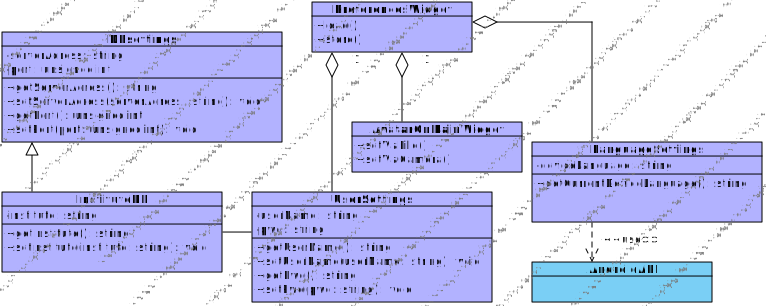
\includegraphics[width=0.8\textwidth]{../grafiken/OptionWidgetB.pdf}
        \end{center}
    \end{block}
}

%%################################################## 

\section{Fazit}
\frame{
\frametitle{Lessons Learned}
	\begin{block}{Was lief gut?}
		\begin{itemize}
			\item erster Punkt
		\end{itemize}
	\end{block}
	\begin{block}{Was lief schlecht?}
		\begin{itemize}
			\item erster Punkt
		\end{itemize}
	\end{block}
}

%%~~~~~~~~~~~~~~~~~~~~~~~~~~~~~~~~~~~~~~~~~~~~~~~~~~~
\frame{
\frametitle{Thank you for your attention}
	\begin{block}{Contact}
	\flushright{
	\tiny Title.\\ \normalsize
	\textbf{Name} \\
	Laboratory of mobile Robotics\\
	Kesslerplatz 12 -- KA 640\\
	90489 Nuremberg \\
	\url{Email40432@ohm-hochschule.de}
	}
	\end{block}	
}

%##################################################
\frame{%\section*{References}
\frametitle{References}
	\begin{block}{Verwendete Software}
			\begin{itemize}
				\item Eclipse Kepler 
				\item Visual Paradigm for UML Professional Edition
			\end{itemize}
	\end{block} 
		
	References

}
\end{document}
